% Options for packages loaded elsewhere
\PassOptionsToPackage{unicode}{hyperref}
\PassOptionsToPackage{hyphens}{url}
%
\documentclass[
]{article}
\usepackage{amsmath,amssymb}
\usepackage{lmodern}
\usepackage{iftex}
\usepackage{graphicx}

\ifPDFTeX
  \usepackage[T1]{fontenc}
  \usepackage[utf8]{inputenc}
  \usepackage{textcomp} % provide euro and other symbols
\else % if luatex or xetex
  \usepackage{unicode-math}
  \defaultfontfeatures{Scale=MatchLowercase}
  \defaultfontfeatures[\rmfamily]{Ligatures=TeX,Scale=1}
\fi
% Use upquote if available, for straight quotes in verbatim environments
\IfFileExists{upquote.sty}{\usepackage{upquote}}{}
\IfFileExists{microtype.sty}{% use microtype if available
  \usepackage[]{microtype}
  \UseMicrotypeSet[protrusion]{basicmath} % disable protrusion for tt fonts
}{}
\makeatletter
\@ifundefined{KOMAClassName}{% if non-KOMA class
  \IfFileExists{parskip.sty}{%
    \usepackage{parskip}
  }{% else
    \setlength{\parindent}{0pt}
    \setlength{\parskip}{6pt plus 2pt minus 1pt}}
}{% if KOMA class
  \KOMAoptions{parskip=half}}
\makeatother
\usepackage{xcolor}
\IfFileExists{xurl.sty}{\usepackage{xurl}}{} % add URL line breaks if available
\IfFileExists{bookmark.sty}{\usepackage{bookmark}}{\usepackage{hyperref}}
\hypersetup{
  pdftitle={arc42 Template},
  hidelinks,
  pdfcreator={LaTeX via pandoc}}
\urlstyle{same} % disable monospaced font for URLs
\usepackage{longtable,booktabs,array}
\usepackage{calc} % for calculating minipage widths
% Correct order of tables after \paragraph or \subparagraph
\usepackage{etoolbox}
\makeatletter
\patchcmd\longtable{\par}{\if@noskipsec\mbox{}\fi\par}{}{}
\makeatother
% Allow footnotes in longtable head/foot
\IfFileExists{footnotehyper.sty}{\usepackage{footnotehyper}}{\usepackage{footnote}}
\makesavenoteenv{longtable}
\usepackage{graphicx}
\makeatletter
\def\maxwidth{\ifdim\Gin@nat@width>\linewidth\linewidth\else\Gin@nat@width\fi}
\def\maxheight{\ifdim\Gin@nat@height>\textheight\textheight\else\Gin@nat@height\fi}
\makeatother
% Scale images if necessary, so that they will not overflow the page
% margins by default, and it is still possible to overwrite the defaults
% using explicit options in \includegraphics[width, height, ...]{}
\setkeys{Gin}{width=\maxwidth,height=\maxheight,keepaspectratio}
% Set default figure placement to htbp
\makeatletter
\def\fps@figure{htbp}
\makeatother
\setlength{\emergencystretch}{3em} % prevent overfull lines
\providecommand{\tightlist}{%
  \setlength{\itemsep}{0pt}\setlength{\parskip}{0pt}}
\setcounter{secnumdepth}{-\maxdimen} % remove section numbering
\ifLuaTeX
  \usepackage{selnolig}  % disable illegal ligatures
\fi

\title{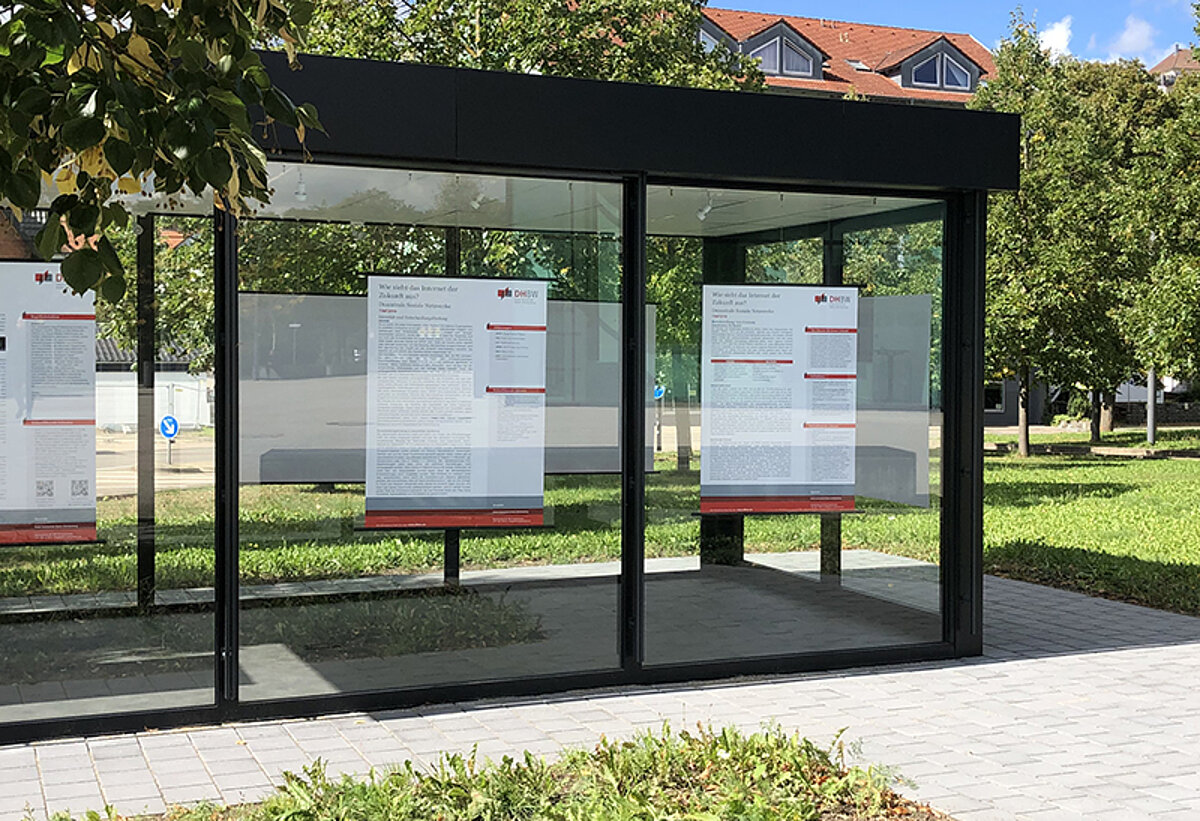
\includegraphics{header.jpg} Template}
\author{}
\date{Januar 2023}
\usepackage{geometry} 

\geometry{
    a4paper,
    left=2cm,
    right=2cm,
    top=2cm,
    bottom=2cm
}
\begin{document}
\maketitle
% DOCUMENT STARTS HERE
\hypertarget{section-introduction-and-goals}{%
\section{Einführung und Ziele}\label{section-introduction-and-goals}}
Die Blickboxen vor der DHBW Heidenheim soll um smarte Features erweitert werden.
Diese sollen dazu dienen die Blickbox attraktiver zu machen.
Außerdem dient das Projekt als Basis für weitere Semesterprojekte der Informatikstudiengänge die Blickbox.
Vor der Implementierung der Features wird eine ausführlich durchdachte Software-Design- und Architekturplanung stattfinden.

Zu den smarten Features gehören:
\begin{itemize}
  \item Überwachung der Wetterdaten
  \item Übermittlung der Daten an zentrale Datenbank
  \item Visualisierung der Daten zur Interaktion mit Dritten
  \item Überwachen des Akkustandes
\end{itemize}




\hypertarget{_stakeholder}{%
\subsection{Stakeholder}\label{_stakeholder}}
Ein umfassender Überblick über die Stakeholder des Systems ist von entscheidender Bedeutung. Dies bezieht sich auf sämtliche Personen, Rollen oder Organisationen, die entweder die Architektur des Systems kennen sollten oder von dieser überzeugt werden müssen. Zu den Stakeholdern zählen auch jene, die aktiv mit der Architektur oder dem Code arbeiten, beispielsweise indem sie Schnittstellen nutzen. Ebenso gehören Personen dazu, die die Dokumentation der Architektur benötigen, um ihre eigene Arbeit effizient zu gestalten. Darüber hinaus sind Stakeholder involviert, die Entscheidungen über das System und dessen Entwicklung treffen.
Die nachfolgende Analyse zeigt alle Stakeholder gebündelt in ihren Gewichtungen und Beziehungen.  
\begin{figure}
  \centering
  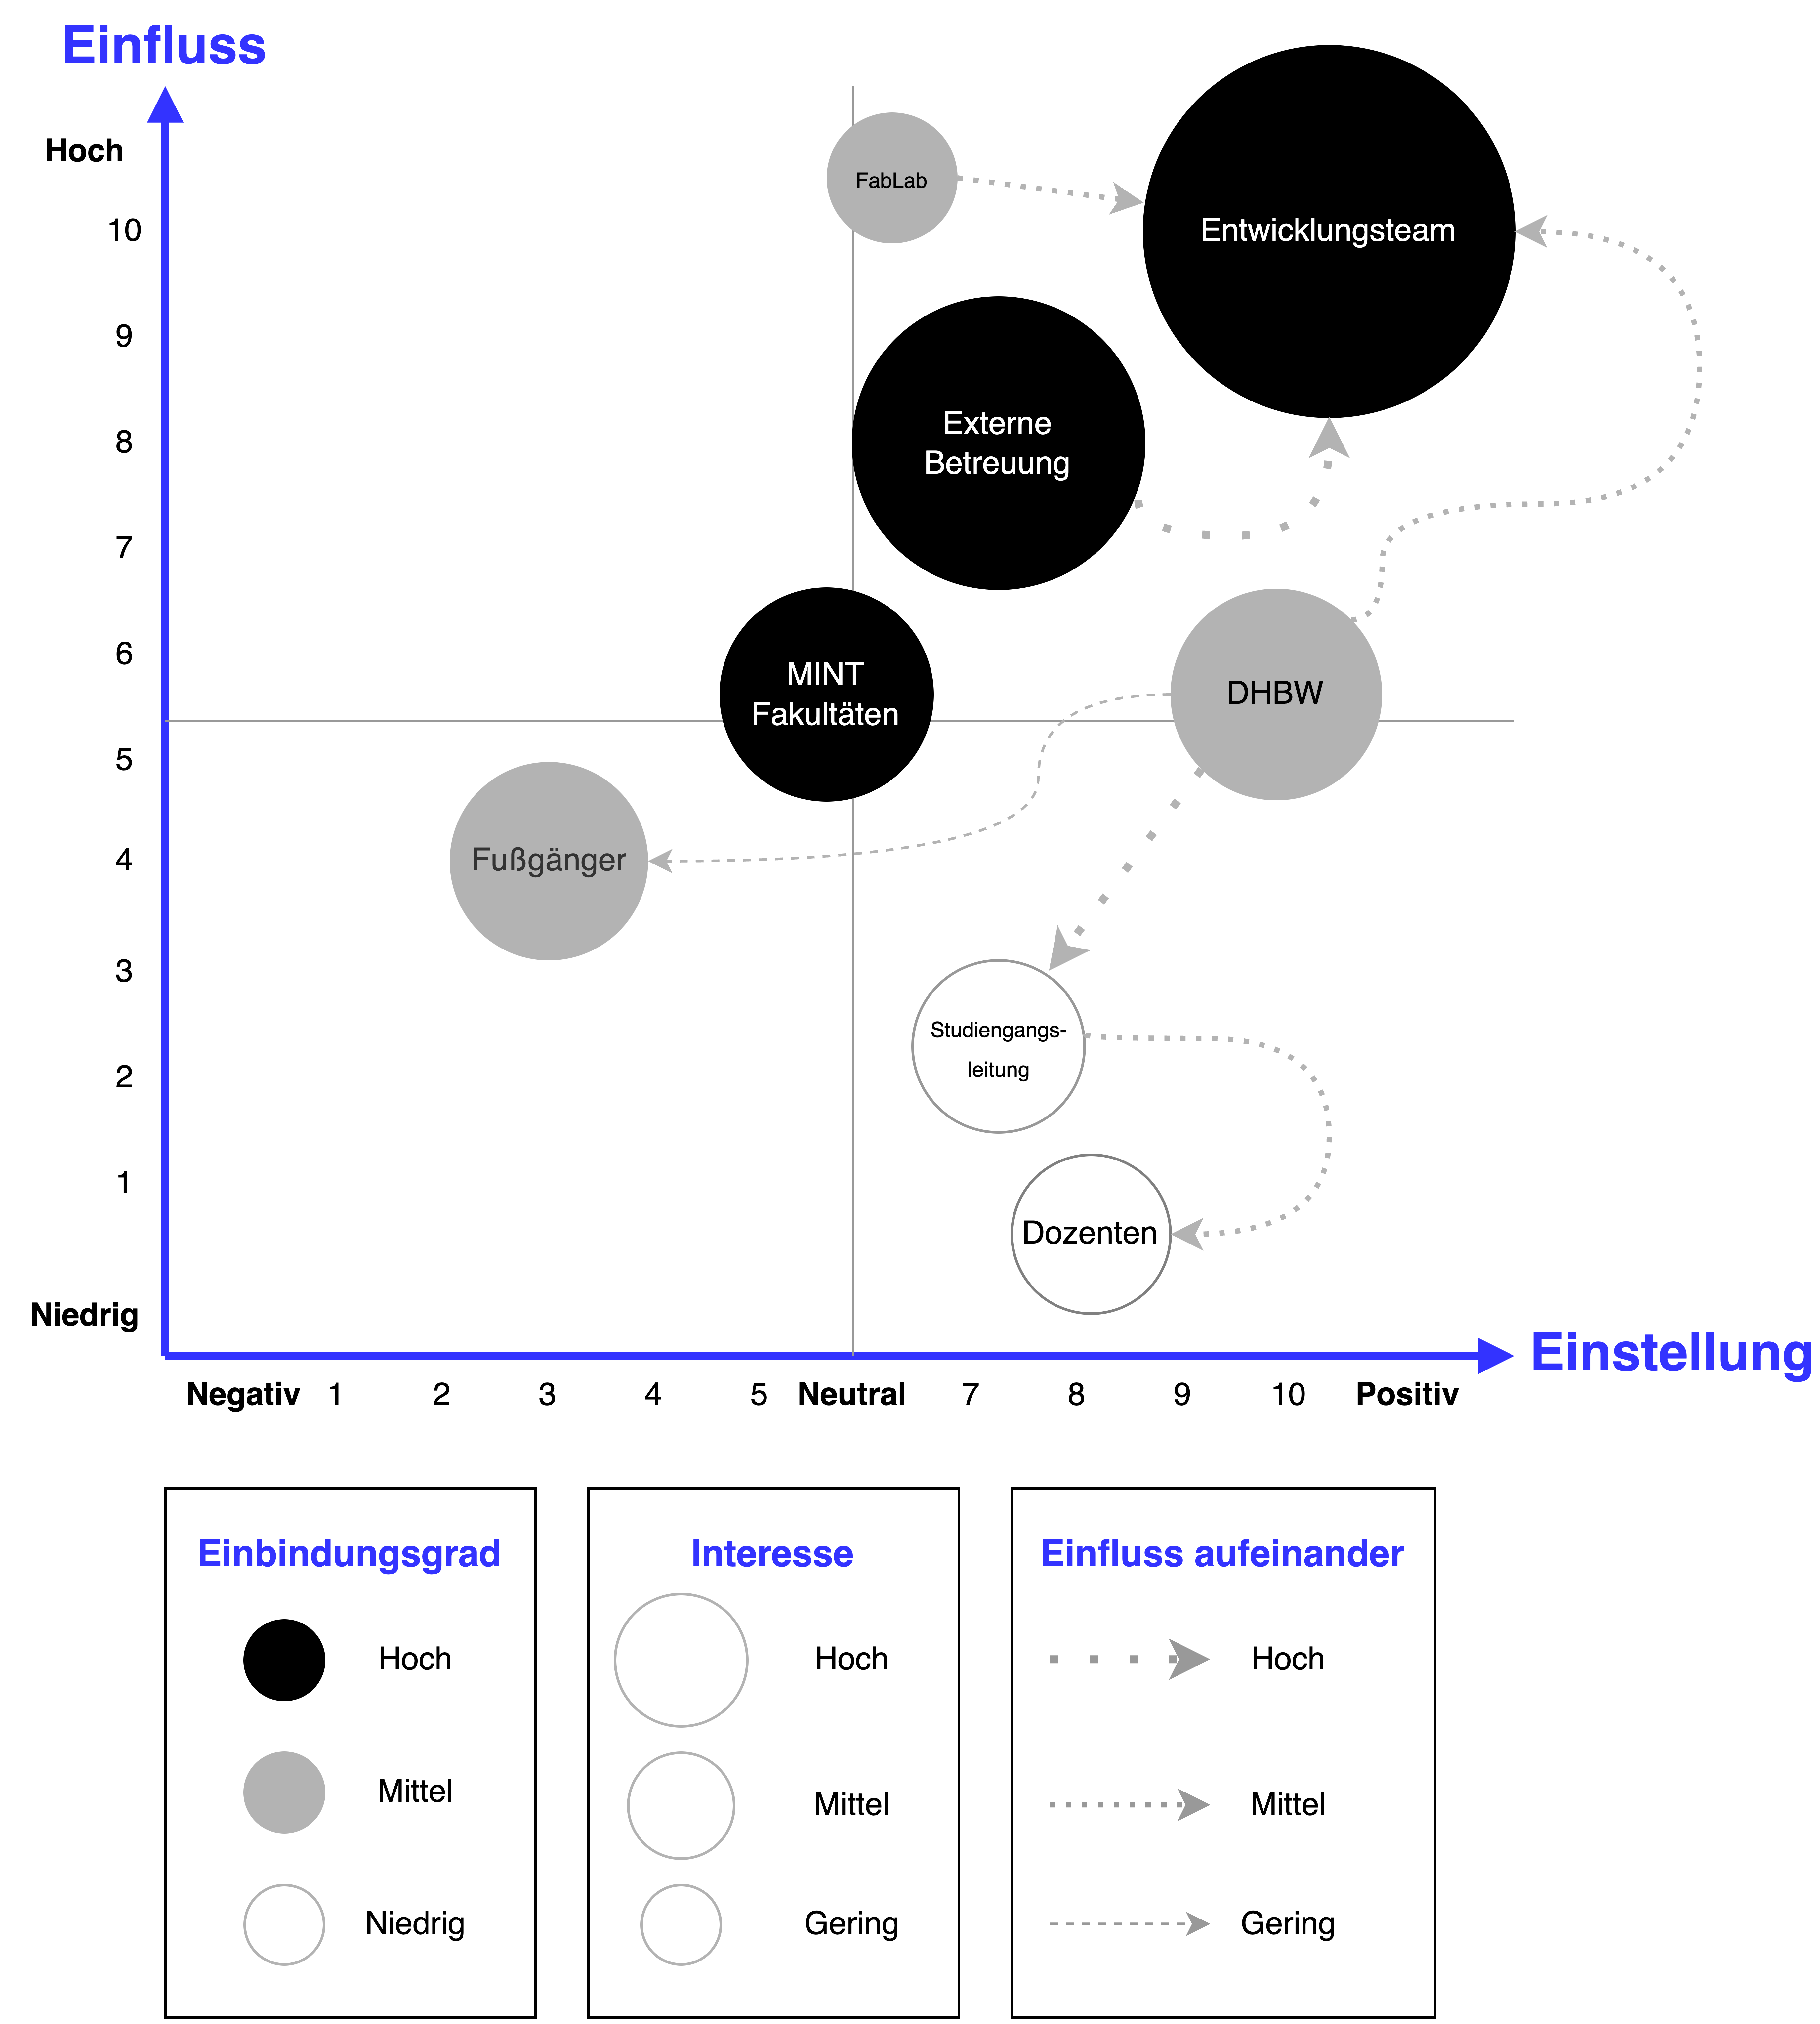
\includegraphics[width=1\textwidth]{./resources/stakeholderanalyse.drawio.png}
  \caption{Stakeholder Analyse und Zusammenfassung in den Unterscheidungen: Einbindungsgrad, Interesse und Einflüsse. Das Entwicklungsteam geht deutlich als am stärksten partizipativ gekennzeichneten Stakeholder hevor. Am repressivsten zeigen sich die Stakeholder in Form der Fußgänger.}
  \label{fig:deine_label}
\end{figure}

\section{Anforderungskonzept}
Die Anforderungen an die Umsetzung des Blickbox-Projekts werden in die Kategorien funktionale, nicht funktionale und hypothetische Anforderungen unterteilt.
Diese Differenzierung ermöglicht eine umfassende Abdeckung aller Aufgabenstellungen im
Zusammenhang mit der Umsetzung des Blickbox-Projekts.

\subsection{Funktionale Anforderungen (FA)}
  Funktionale Anforderungen beschreiben spezifisch die konkreten Zwecke, die das zu entwickelnde Produkt erfüllen soll.

\subsection{Nicht funktionale Anforderungen (NFA)}
Im Gegensatz zu funktionalen Anforderungen sind nicht-funktionale Anforderungen eher allgemein gehalten und betreen die gesamte Architektur und das Design des Produkts.
Sie können auf verschiedene Projekte angewendet werden.

\subsection{Hyptohetische Anforderungen (HFA)}
Hypothetische Anforderungen werden aufgrund von unsicheren Ergebnissen und vorherigen Abhängigkeiten definiert. Ihr Zweck besteht darin, mögliche Entscheidungen und Eventualitäten abzudecken, die eintreten können oder auch nicht.


\begin{center}
  \begin{tabular}{|p{\linewidth}|}
    \hline
    \textbf{Datenerfassung und -übertragung (FA1)} \\
    Beschreibung: Das IOT-System muss in der Lage sein, kontinuierlich Sensordaten zu erfassen.
    Diese Daten sollen in der Sensoreinheit eingelesen und im Raspberry PI gespeichert und verarbeitet werden.
    Die Datenübertragung auf den Server erfolgt Event-gesteuert und drahtlos über einen http-Client.
    Die Daten werden in festgelegten Intervallen im JSON-Format übertragen und in der Datenbank festgehalten. \\ \\
    \hline
    \textbf{Interaktivität zu Dritten (FA2)} \\
    Beschreibung: Der Blickbox soll attraktiver werden und Fußgänger sollen mit ihm interagieren können.
    Das soll in Form eines Displays oder Ton und Licht geschehen.
    Ein Display soll in der Lage sein, Dritten aktuelle Daten aus der Datenbank wie etwa das Wetter anzuzeigen.
    Bei Dunkelheit sollen Bewegungsmelder Lichter aktivieren.\\ \\
    \hline
    \textbf{Containerisierung (FA3)} \\
    Beschreibung: Die Anwendungen sollen in Containern gekapselt werden, um eine verbesserte Portabilität und Skalierbarkeit zu gewährleisten.
    Es wird die Container-Technologien Docker verwendet werden, um die Anwendungen effizient zu verwalten und zu deployen. \\ \\
    \hline
  \end{tabular}
\end{center}

\begin{center}
  \begin{tabular}{|p{\linewidth}|}
    \hline
    \textbf{Erweiterbarkeit und Wartung (NF1)} \\
    Beschreibung: Die Architektur und Dokumentation des Systems sollen leicht zugänglich sein, um Erweiterungen und Verbesserungen der Features zu erleichtern.
    Eine klare Dokumentation sowie ein vereinfachter Hardwareaufbau sollen die Wartung und Erweiterbarkeit des Systems unterstützen. \\ \\
    \hline
    \textbf{Sicherheit (NF2)} \\
    Beschreibung: Die Verbindung zum Server soll verschlüsselt sein, um die Sicherheit der übertragenen Daten zu gewährleisten.
    Es müssen geeignete Verschlüsselungsprotokolle und Sicherheitsmaßnahmen implementiert werden, um die Vertraulichkeit und Integrität der Daten zu schützen.\\ \\
    \hline
    \textbf{Datenwiederherstellung und -erhaltung (NF3)} \\
    Beschreibung: Ein Standardprogramm auf dem Raspberry Pi soll die kontinuierliche Sicherung der Daten gewährleisten, um die ungestörte Funktionalität der Blickbox zu sichern.
    Die Daten puffern wir auf dem Pi, damit die Datenbank nur zur Darstellung in Grafana existiert.
    Die Daten sollen dazu auf dem Raspberry Pi in einer Datei gespeichert werden.
    Das Risiko des Verlierens der Daten soll so minimiert werden.\\ \\
    \hline
    \textbf{Bereitstellung einer geeigneten Umgebung für die Hardware (NF4)} \\
    Beschreibung: Die Hardware muss sowohl innerhalb als auch außerhalb der Blickbox an trockenen und sicheren Orten platziert werden.
    Es sollen wetterfeste und isolierte Boxen verwendet werden, um die Hardware vor Umwelteinflüssen zu schützen und ihre Langlebigkeit zu gewährleisten.\\ \\
    \hline
    \textbf{Bereitstellung eines Dashboard (NF5)} \\
    Beschreibung: Die Daten der Datenbank sollen mit Grafana grafisch dargestellt werden.
    Auf dem Dashboard sollen die Grafana-Grafen visualisiert werden und den Verbindungsstatus zur Datenbank sowie zur Blickbox angegeben werden.
    Es soll nutzerfreundlich sein, um die Datenvisualisierung für Benutzer intuitiv zugänglich zu machen.
    \\ \\
    \hline
  \end{tabular}
\end{center}



\newpage
\section{Randbedingungen}
\subsection{Technisch}
\begin{longtable}[]{@{}
  >{\raggedright\arraybackslash}p{(\columnwidth - 4\tabcolsep) * \real{0.2500}}
  >{\raggedright\arraybackslash}p{(\columnwidth - 4\tabcolsep) * \real{0.7500}}@{}}
\toprule
\begin{minipage}[b]{\linewidth}\raggedright
Randbedingung
\end{minipage} & \begin{minipage}[b]{\linewidth}\raggedright
Beschreibung
\end{minipage} \\
\midrule
\endhead
Datenbank &
Zur Datenbankpersistenz wird eine NoSQL-Datenbank wie InfluxDB verwendet. \\
Datenübertragung & 
Die Wetterstation wird über das Internet (WLAN) mit einer API kommunizieren. \\
Aufteilung & 
Frontend und Backend werden strikt getrennt. \\
 &\\
Fremdsoftware & 
Opensource Bibiliotheken dürfen verwendet werden.\\
 &\\
Wasserfestigkeit & 
Jegliche Hardware muss Wasserfest implementiert werden.\\
\bottomrule
\end{longtable}

\subsection{Organisatorisch}
\begin{longtable}[]{@{}
  >{\raggedright\arraybackslash}p{(\columnwidth - 4\tabcolsep) * \real{0.2500}}
  >{\raggedright\arraybackslash}p{(\columnwidth - 4\tabcolsep) * \real{0.7500}}@{}}
\toprule
\begin{minipage}[b]{\linewidth}\raggedright
Randbedingung
\end{minipage} & \begin{minipage}[b]{\linewidth}\raggedright
Beschreibung
\end{minipage} \\
\midrule
\endhead
Team &
Vivian Berger, Maylis Grune, Max Müller und Aron Seidl \\
Zeitplan &
Der Zeitplan wird auf 2 Monate vom 01.02.2024 - 28.03.2024 festgelegt. \\
 &\\
Projektmanagement & 
Die Entwicklung folgt dem Scrum-Framework mit zweiwöchigen Sprints. \\
Definition of Done &
Entwickler folgen der DoD auf dem Git-Repository. \\
\bottomrule
\end{longtable}


\newpage
\section{Kontextabgrenzung}
\subsection{Fachlicher Kontext}
\begin{figure}[htbp]
	\centering
	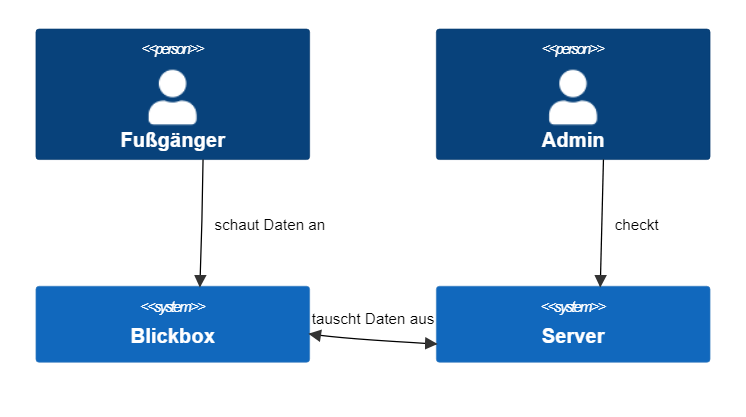
\includegraphics[width=140mm]{../c4/Business_Context.png}
	\caption{Kontextdiagramm Blickbox }
	\label{fig:Kontextdiagramm}
\end{figure}  

\begin{longtable}[]{@{}
  >{\raggedright\arraybackslash}p{(\columnwidth - 4\tabcolsep) * \real{0.2500}}
  >{\raggedright\arraybackslash}p{(\columnwidth - 4\tabcolsep) * \real{0.7500}}@{}}
\toprule
\begin{minipage}[b]{\linewidth}\raggedright
Knoten
\end{minipage} & \begin{minipage}[b]{\linewidth}\raggedright
Beschreibung
\end{minipage} \\
\midrule
\endhead
Fußgänger &
Fußgänger die sich die Blickbox anschauen und die Daten sehen. \\
Admin &
Administriert Dashboards und stuert Blickbox manuell. \\
 & \\
Blickbox & 
Enthält Sensor Hardware und Anzeige der Daten. \\
 & \\
Server &
Externer Server der mit der Hardware der Blickbox kommuniziert. \\
\bottomrule
\end{longtable}
\newpage
\subsection{Technischer Kontext}
\begin{figure}[htbp]
	\centering
	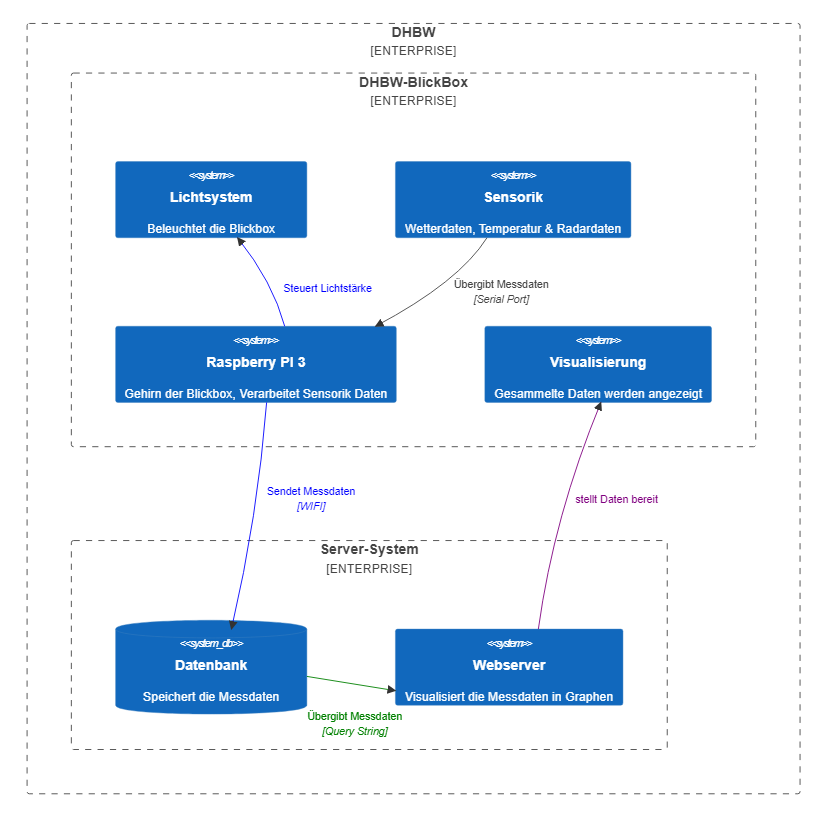
\includegraphics[width=125mm]{../c4/Technical_Context.png}
	\caption{Kontextdiagramm Blickbox }
	\label{fig:Kontextdiagramm}
\end{figure}  

\begin{longtable}[]{@{}
  >{\raggedright\arraybackslash}p{(\columnwidth - 4\tabcolsep) * \real{0.2500}}
  >{\raggedright\arraybackslash}p{(\columnwidth - 4\tabcolsep) * \real{0.7500}}@{}}
\toprule
\begin{minipage}[b]{\linewidth}\raggedright
Knoten
\end{minipage} & \begin{minipage}[b]{\linewidth}\raggedright
Beschreibung
\end{minipage} \\
\midrule
\endhead
Lichtsystem &
Beleuchtet die Blickbox. \\
Sensorik &
Hardware welche die Messdaten sammelt. \\
 &\\
RaspberryPI & 
Verarbeitet die Sensorik Daten und schickt diese an die Datenbank. \\
Visualisierung &
Gesammelte Daten werden angezeigt. \\
Datenbank &
Speichert die Messdaten. \\
Webserver & 
Visualisiert die Messdaten und Stellt Frontend bereit. \\
\bottomrule
\end{longtable}



\section{Lösungsstrategie}
\begin{longtable}[]{@{}
  >{\raggedright\arraybackslash}p{(\columnwidth - 4\tabcolsep) * \real{0.2500}}
  >{\raggedright\arraybackslash}p{(\columnwidth - 4\tabcolsep) * \real{0.3000}}
  >{\raggedright\arraybackslash}p{(\columnwidth - 4\tabcolsep) * \real{0.4000}}@{}}
\toprule
\begin{minipage}[b]{\linewidth}\raggedright
Ziel / Requirement
\end{minipage} & \begin{minipage}[b]{\linewidth}\raggedright
Lösungsstrategie
\end{minipage} & \begin{minipage}[b]{\linewidth}\raggedright
Details
\end{minipage} \\
\midrule
\endhead
Alle funktionalen Requirements &
Eventgesteuerte Architektur &
Sensorarchitektur sendet die Messdaten an dem PI. Der PI sendet die Daten an den Webserver über das Internet, da LoraWan ineffizient ist. Der Webserver speichert diese ab und stellt diese im Frontend da.\\
& & \\
Erweitbarkeit \& Wartung  &
Modularer Projektaufbau und Tests &
Damit Dritte, sei es irgendwelche Stakeholder oder neue Entwickler, sich in das Projekt leicht einarbeiten können, bauen wir das Projekt so auf, dass Codecomponenten voneinander getrennt aufgebaut sind, sich also in Modulen befinden. Zudem sind Funktionen getestet. \\
& & \\
Sicherheit  &
Https-Verbindung, Containerisierung \& Reverse-Proxy &
Über den Reverse-Proxy sind die Verschiedenen Server-Apps nicht direkt dem Internet Exposed. Durch die Containersierung können die Komponenten innerhalb des Containers kommunizieren. Die verschiedenen Ports können also verschlossen sein. \\
& & \\
Wiederherstellung und -erhaltung der Daten  &
 &
Auf dem Pi werden in einer history file, die daten abgelegt, damit man sollte die verbindung abbrechen, die noch seperat auf dem Pi sind. \\
& & \\
Bereitstellung einer geeigneten Umgebung für die Hardware  &
Box &
SARA wird in einer Box einbaut, welche Wasserdicht ist. Durch eine eigene Batterie ist sie Autak und braucht keine Spannung von außen. Die Sensoren werden über Kabelverschraubung in den Innenraum der Box gebraucht dadurch ist sie Wasserdicht. \\
& & \\
Bereitstellung eines Dashboard  &
Grafana als Open-Source Fertiglösung &
Das erlaubt eine einfache Darstellung der Messdaten mit direkter Datenbank-anbindung, sowie eine einfache Verknüpfung mit dem Frontend. \\
\bottomrule
\end{longtable}
\newpage
\section{Bausteinsicht}

\subsection{Native React App}
\begin{figure}[htbp]
	\centering
	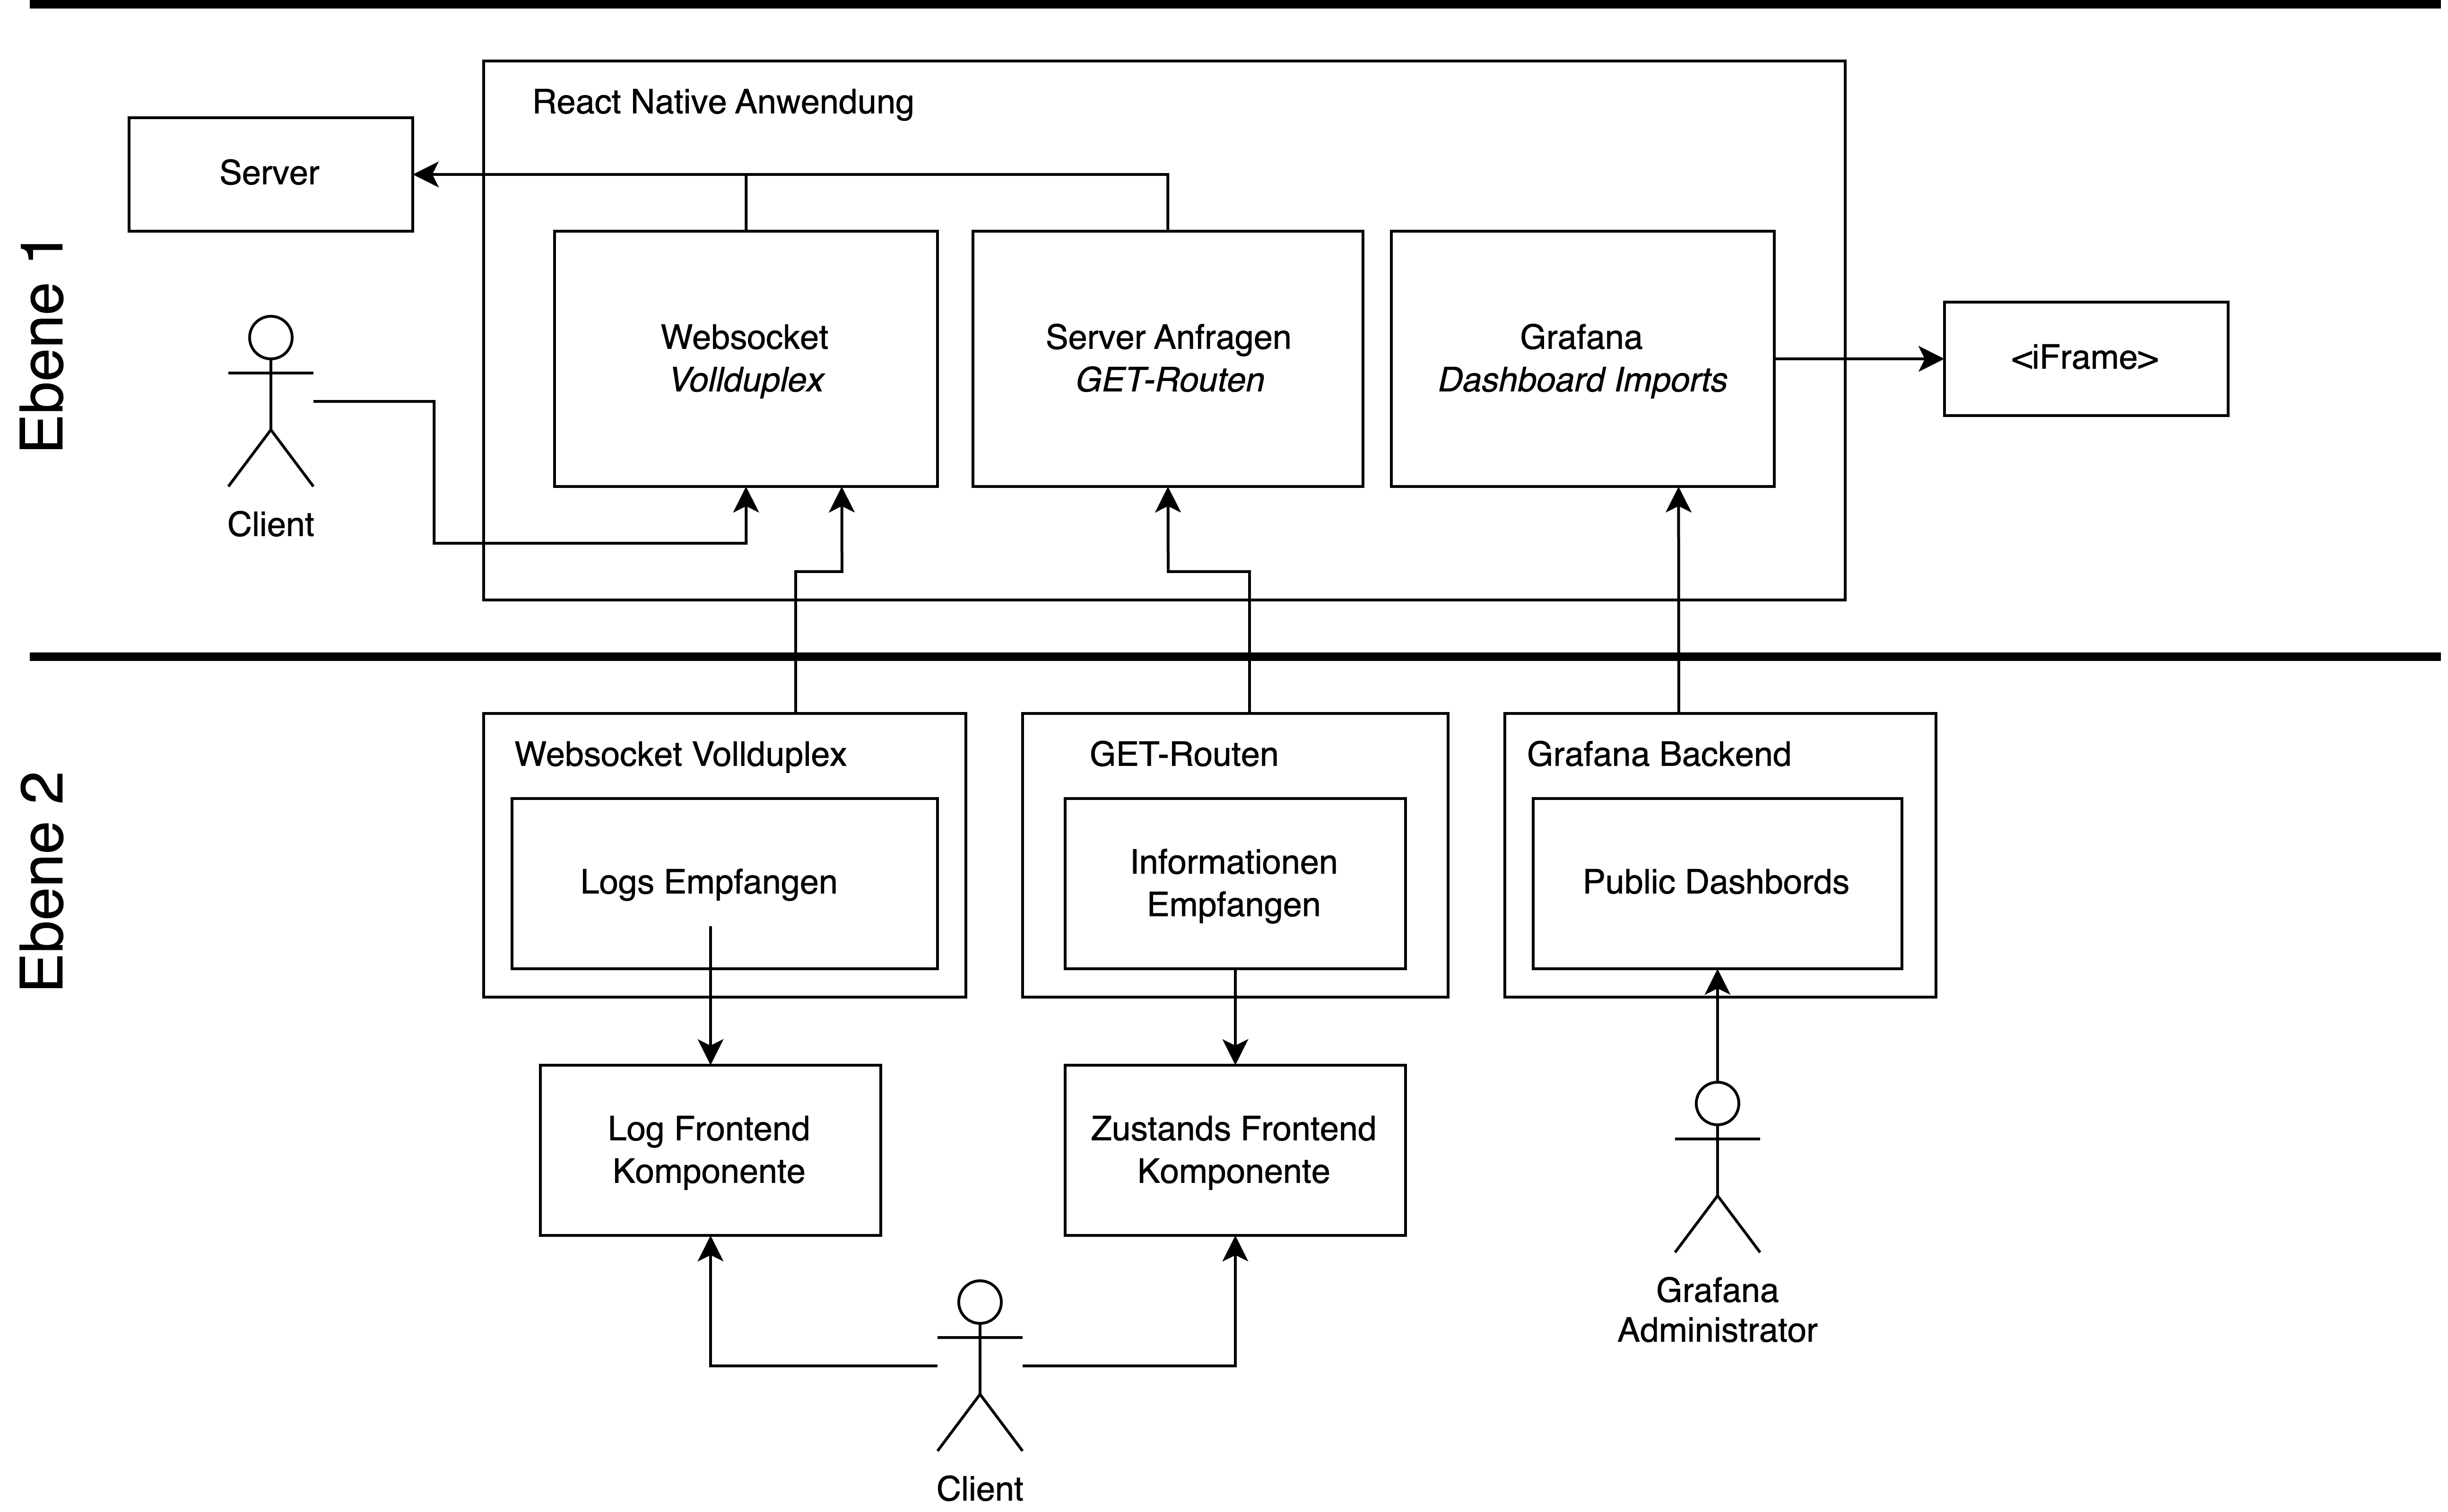
\includegraphics[width=120mm]{resources/BausteinsichtValentin.drawio.png}
	\caption{Bausteinsicht React App}
	\label{fig:ContextDiagram}
\end{figure}  

\subsection{Raspberry PI}
\begin{figure}[htbp]
	\centering
	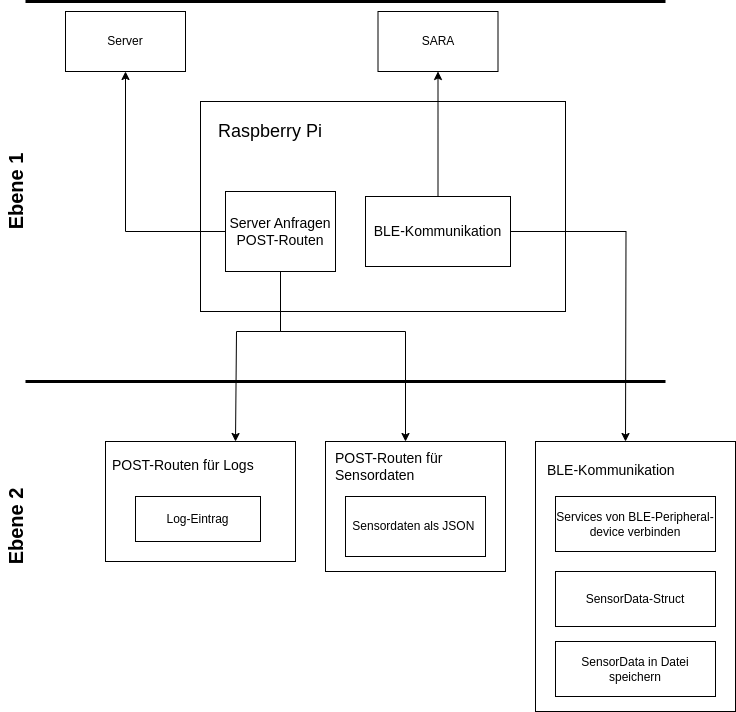
\includegraphics[width=100mm]{resources/ADABausteinsicht.png}
	\caption{Bausteinsicht Raspberry PI}
	\label{fig:ContextDiagram}
\end{figure}  
\newpage
\subsection{Sensorik}
\begin{figure}[htbp]
	\centering
	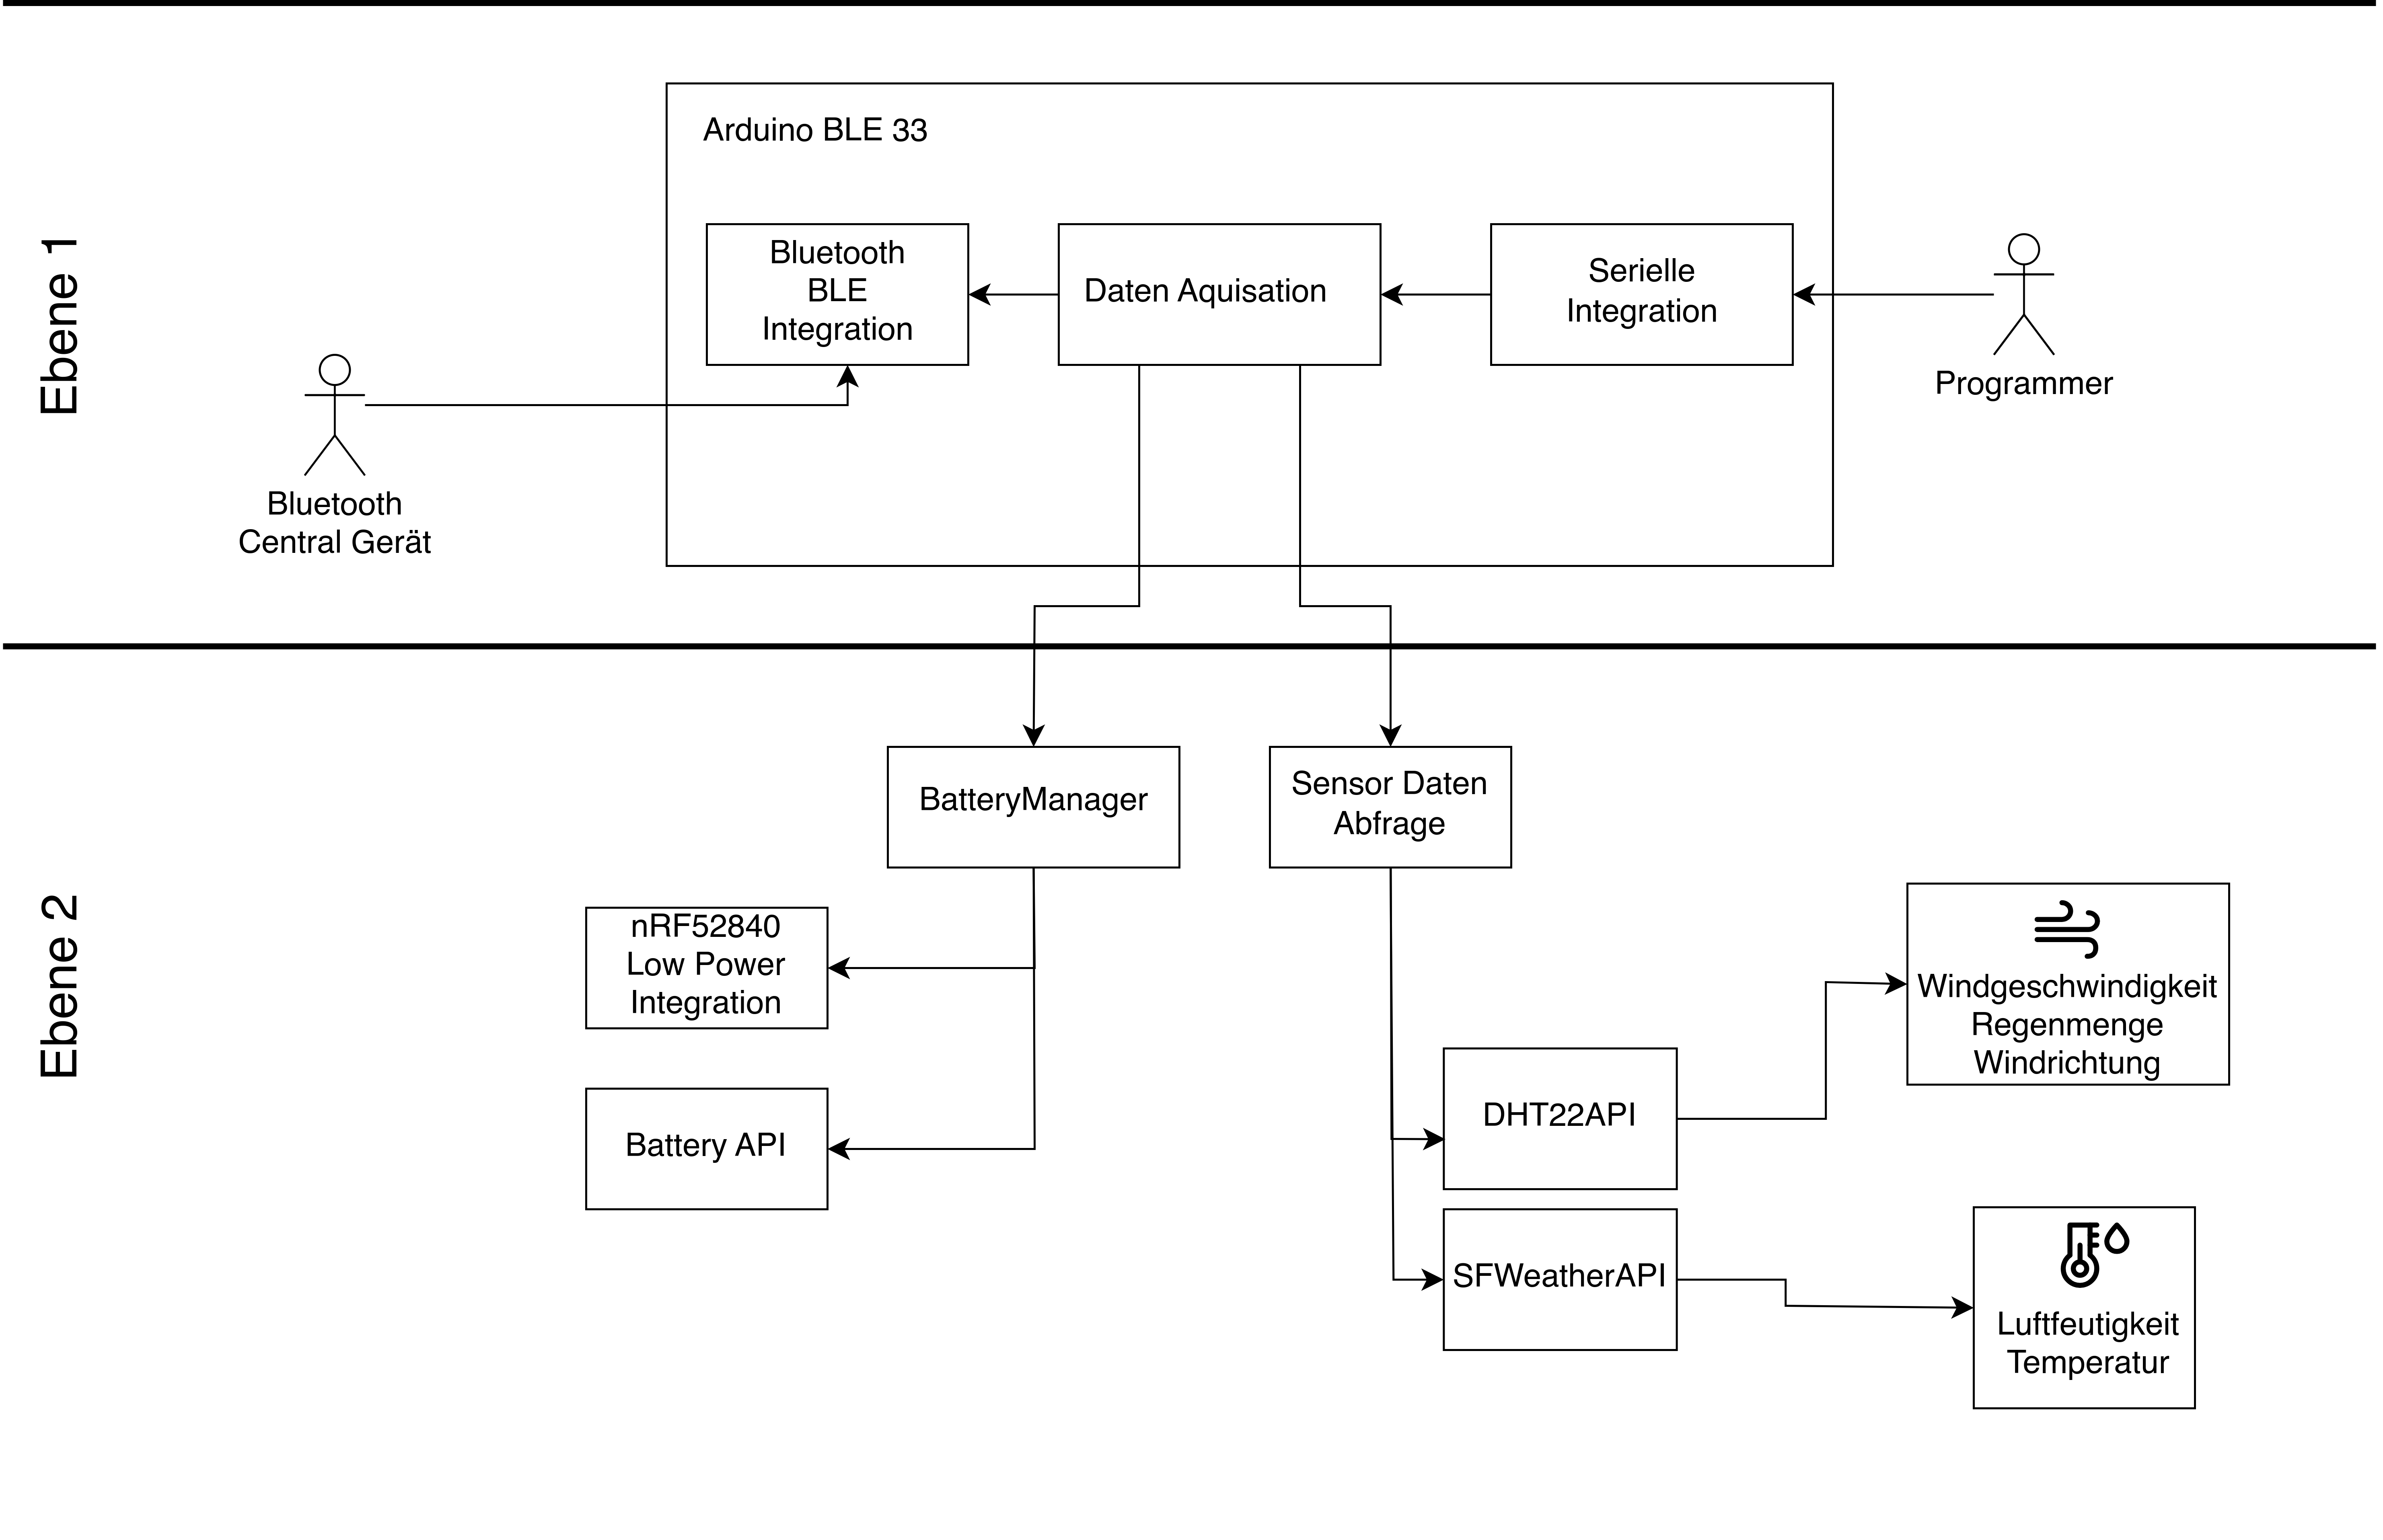
\includegraphics[width=130mm]{resources/Bausteinschicht_Sara.png}
	\caption{Bausteinsicht Server}
	\label{fig:ContextDiagram}
\end{figure}  
\subsection{Server}
\begin{figure}[htbp]
	\centering
	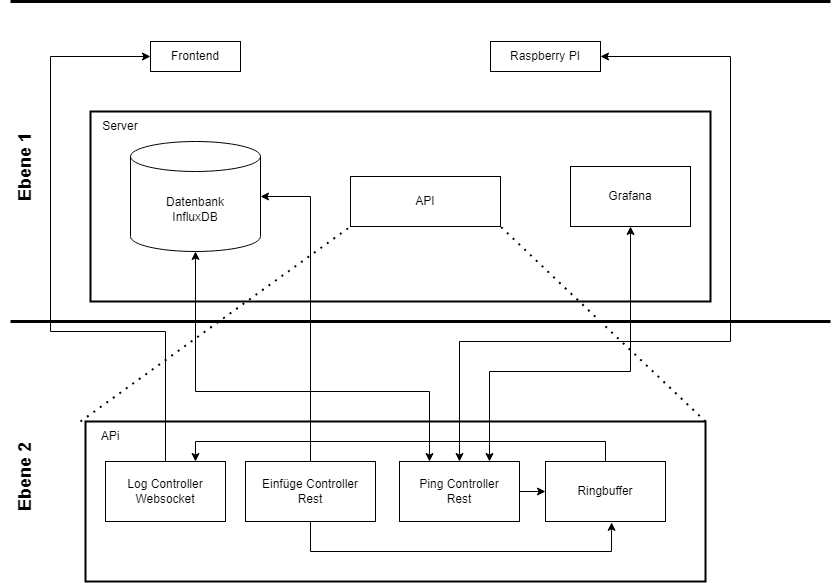
\includegraphics[width=130mm]{resources/Bausteinsicht_Server.png}
	\caption{Bausteinsicht Arduino}
	\label{fig:ContextDiagram}
\end{figure}  

\section{Laufzeitsicht}

\section{Verteilungssicht}

\section{Architekturentscheidungen}
\subsection{Evaluation zur Wahl des Frontend-Frameworks des Clients}

Der Client zur Anzeige und Aufbereitung der Sensordaten wird unter dem Arbeitstitel \textit{Valentin} (Komposita aus \textit{Value} und \textit{Notification}) geführt. Vor der Initialisierung von \textit{Valentin} muss ein geeignetes Framework gewählt werden. Die nachfolgende Nutzwertanalyse dient dafür als Entscheidungsgrundlage. 

\begin{figure}
  \centering
  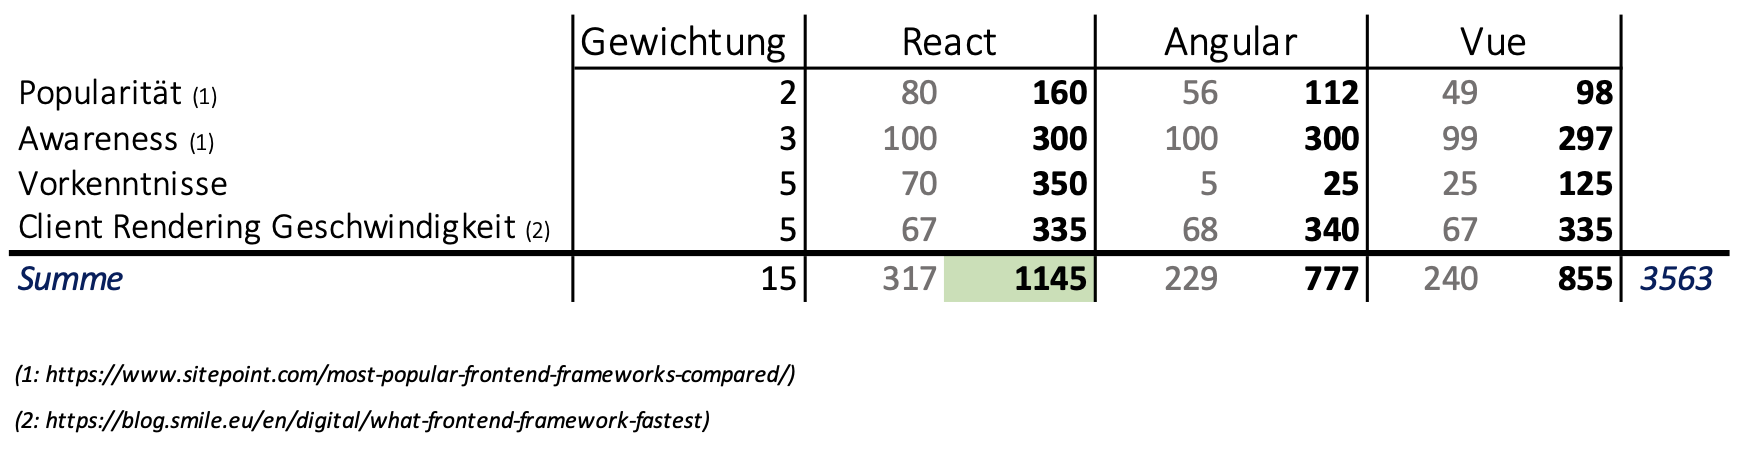
\includegraphics[width=1\textwidth]{./resources/techevaluationfe.png}
  \caption{Nutzwertanalyse zur Entscheidung eines geeigneten Frameworks gemessen an der Popularität, der Entwickler Awarness (Welches Framework enthält welchen Support), den Vorkenntnissen des Entwicklungsteams und der Rendergeschwindigkeit auf den Systemen der Clients.}
  \label{fig:deine_label}
\end{figure}

Die Auswahl zum Framework innerhalb des \textit{Valentin} Client Aufbaus viel auf \textit{React}. \textit{React} ist eine JavaScript-Bibliothek von Facebook für die Entwicklung von interaktiven, komponentenbasierten Benutzeroberflächen. Sie ermöglicht eine effiziente Aktualisierung des DOM und eine verbesserte Leistung durch die Verwendung einer virtuellen DOM-Repräsentation.

\section{Qualitätsanforderungen}
\begin{figure}[htbp]
	\centering
	\includegraphics[width=170mm]{resources/Qualitätsbaum.drawio.png}
	\caption{Qualitätsbaum}
	\label{fig:ContextDiagram}
\end{figure}  

\section{Risiken und Teschnische Schulden}
\section{Glossar}

\end{document}
